\documentclass{beamer}
\usepackage{amsmath}
\usepackage{amssymb}
\usepackage{graphicx}
\usepackage{multicol}
\usepackage{circuitikz}
\usepackage{hyperref}
\usepackage{rotating}
\usepackage{caption}
\usepackage{subcaption}
\usepackage{circuitikz}
\usepackage{tikz}
\title{Übungsgruppe 4: Technische Informatik}
\subtitle{Blatt 11}
\author{Tutor: Gabriella Frank}
\date{19.07.2023}
\begin{document}
\begin{frame}
\titlepage
\end{frame}
\newcommand{\unsim}{\mathord{\sim}}
    \begin{frame}{Aufgabe 2}{}
        \begin{block}{Aufgabe}
            Mealy-Automat gegeben durch:
            \begin{itemize}
                \item $M = (\{0,1\}, \{0,1\}, \{s_1, ..., s_6\}, \{s_1\}, \delta, \lambda)$
            \end{itemize}
            \includegraphics[scale=0.3]{./figures/Mealy-Übergangstafel.png}
        \end{block}
    \end{frame}

    \begin{frame}{Aufgabe 2a}{}
        \begin{block}{Aufgabe} Zustandsdiagramm zeichnen
        \end{block}
        \begin{block}{Lösung}
            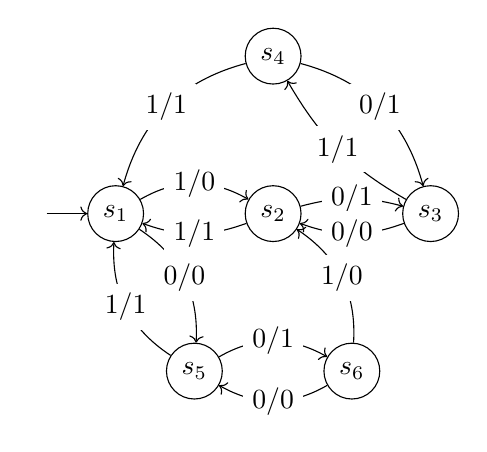
\begin{tikzpicture}[main/.style = {draw, circle}]
            \node[main](1) at (0,0) {$s_1$};
            \node[left of=1](s){};

            \node[main](2) at (2,0) {$s_2$};
            \node[main](3) at (4,0) {$s_3$};
            \node[main](4) at (2,2) {$s_4$};
            \node[main](5) at (1,-2) {$s_5$};
            \node[main](6) at (3,-2) {$s_6$};

            \draw[->] (s) to (1);
            \draw[->] (1) to [bend left = 30] node[midway, fill= white] {1/0} (2);
            \draw[->] (1) to [bend left = 30] node[midway, fill= white] {0/0} (5);
            \draw[->] (2) to [bend left = 20] node[midway, fill= white] {1/1} (1);
            \draw[->] (2) to [bend left = 15] node[midway, fill= white] {0/1} (3);
            \draw[->] (3) to [bend left = 15] node[midway, fill= white] {1/1} (4);
            \draw[->] (3) to [bend left = 20] node[midway, fill= white] {0/0} (2);
            \draw[->] (4) to [bend right = 30] node[midway, fill= white] {1/1} (1);
            \draw[->] (4) to [bend left = 30] node[midway, fill= white] {0/1} (3);
            \draw[->] (5) to [bend left = 30] node[midway, fill= white] {1/1} (1);
            \draw[->] (5) to [bend left = 30] node[midway, fill= white] {0/1} (6);
            \draw[->] (6) to [bend right = 30] node[midway, fill= white] {1/0} (2);
            \draw[->] (6) to [bend left = 30] node[midway, fill= white] {0/0} (5);
            \end{tikzpicture}
        \end{block}
    \end{frame}

    \begin{frame}{Aufgabe 2b}{}
        Äquivalente Zustände: Bei gleicher Eingabe - gleiche Ausgabe und gleicher Folgezustand\\
        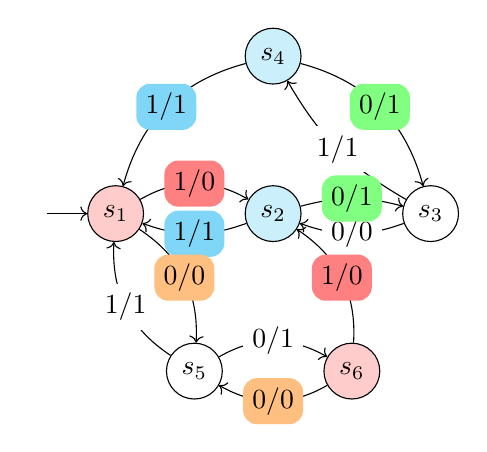
\begin{tikzpicture}[main/.style = {draw, circle}]
            \node[main, fill=red!20](1) at (0,0) {$s_1$};
            \node[left of=1](s){};

            \node[main, fill=cyan!20](2) at (2,0) {$s_2$};
            \node[main](3) at (4,0) {$s_3$};
            \node[main, fill=cyan!20](4) at (2,2) {$s_4$};
            \node[main](5) at (1,-2) {$s_5$};
            \node[main, fill=red!20](6) at (3,-2) {$s_6$};

            \draw[->] (s) to (1);
            \draw[->] (1) to [bend left = 30] node[midway, fill= red!50, rounded corners=5pt] {1/0} (2);
            \draw[->] (2) to [bend left = 20] node[midway, fill= cyan!50, rounded corners=5pt] {1/1} (1);
            \draw[->] (3) to [bend left = 15] node[midway, fill= white] {1/1} (4);
            \draw[->] (3) to [bend left = 20] node[midway, fill= white] {0/0} (2);
            \draw[->] (4) to [bend right = 30] node[midway, fill= cyan!50, rounded corners=5pt] {1/1} (1);
            \draw[->] (4) to [bend left = 30] node[midway, fill= green!50, rounded corners=5pt] {0/1} (3);
            \draw[->] (5) to [bend left = 30] node[midway, fill= white] {1/1} (1);
            \draw[->] (5) to [bend left = 30] node[midway, fill= white] {0/1} (6);
            \draw[->] (6) to [bend right = 30] node[midway, fill= red!50, rounded corners=5pt] {1/0} (2);
            \draw[->] (6) to [bend left = 30] node[midway, fill= orange!50, rounded corners=5pt] {0/0} (5);
            \draw[->] (1) to [bend left = 30] node[midway, fill= orange!50, rounded corners=5pt] {0/0} (5);
            \draw[->] (2) to [bend left = 15] node[midway, fill= green!50, rounded corners=5pt] {0/1} (3);
            \end{tikzpicture}
    \end{frame}

    \begin{frame}{Aufgabe 2b}
        \begin{block}{Lösung}
        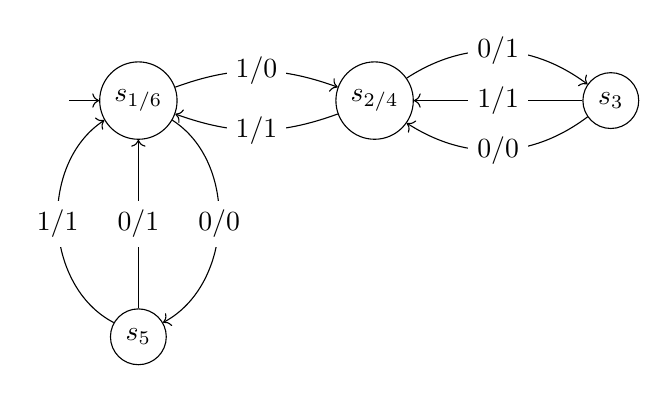
\begin{tikzpicture}[main/.style = {draw, circle}]
            \node[main](1) at (0,0) {$s_{1/6}$};
            \node[left of=1](s){};

            \node[main](2) at (3,0) {$s_{2/4}$};
            \node[main](3) at (6,0) {$s_3$};
            \node[main](5) at (0,-3) {$s_5$};

            \draw[->] (s) to (1);
            \draw[->] (1) to [bend left = 20] node[midway, fill= white] {1/0} (2);
            \draw[->] (1) to [bend left = 60] node[midway, fill= white] {0/0} (5);
            \draw[->] (2) to [bend left = 20] node[midway, fill= white] {1/1} (1);
            \draw[->] (2) to [bend left = 35] node[midway, fill= white] {0/1} (3);
            \draw[->] (3) to node[midway, fill= white] {1/1} (2);
            \draw[->] (3) to [bend left = 35] node[midway, fill= white] {0/0} (2);
            \draw[->] (5) to [bend left = 60] node[midway, fill= white] {1/1} (1);
            \draw[->] (5) to node[midway, fill= white] {0/1} (1);
            \end{tikzpicture}
        \end{block}
    \end{frame}

    \begin{frame}{Aufgabe 2c}{}
        \begin{itemize}
            \item Zustandscodierung
            \item Zustands- und Ausgangstafel
        \end{itemize}
        \begin{block}{Lösung}
        \begin{itemize}
            \item $s_{i} = (z_1, z_0), s_{1,6} = (0, 0), s_{2,4} = (0, 1), s_{3} = (1, 0), s_{5} = (1, 1)$
            \item \includegraphics[scale=0.3]{./figures/Mealy-reduziert-Übergangstafel.png}
        \end{itemize}
        \end{block}
    \end{frame}

    \begin{frame}{Aufgabe 2d}{}
      \begin{columns}
        \begin{column}{0.5\textwidth}
            \begin{block}{Aufgabe}
                \begin{itemize}
                    \item Übergangsfunktionen
                    \item Ausgangsfunktion
                    \item Schaltwerk
                    \item \includegraphics[scale=0.12]{./figures/Mealy-reduziert-Übergangstafel-Funktionen.png}
                \end{itemize}
            \end{block}
        \end{column}
        \begin{column}{0.5\textwidth}
            \begin{block}{Lösung}
                \begin{itemize}
                    \item $z_0^{t+1} = \overline{z}_0^t$
                    \item $z_1^{t+1} = \overline{x + z_1^t} = \overline{x} \cdot \overline{z}_1^t$
                    \item $y = z_0^t + x \cdot z_1^t$
                    \item 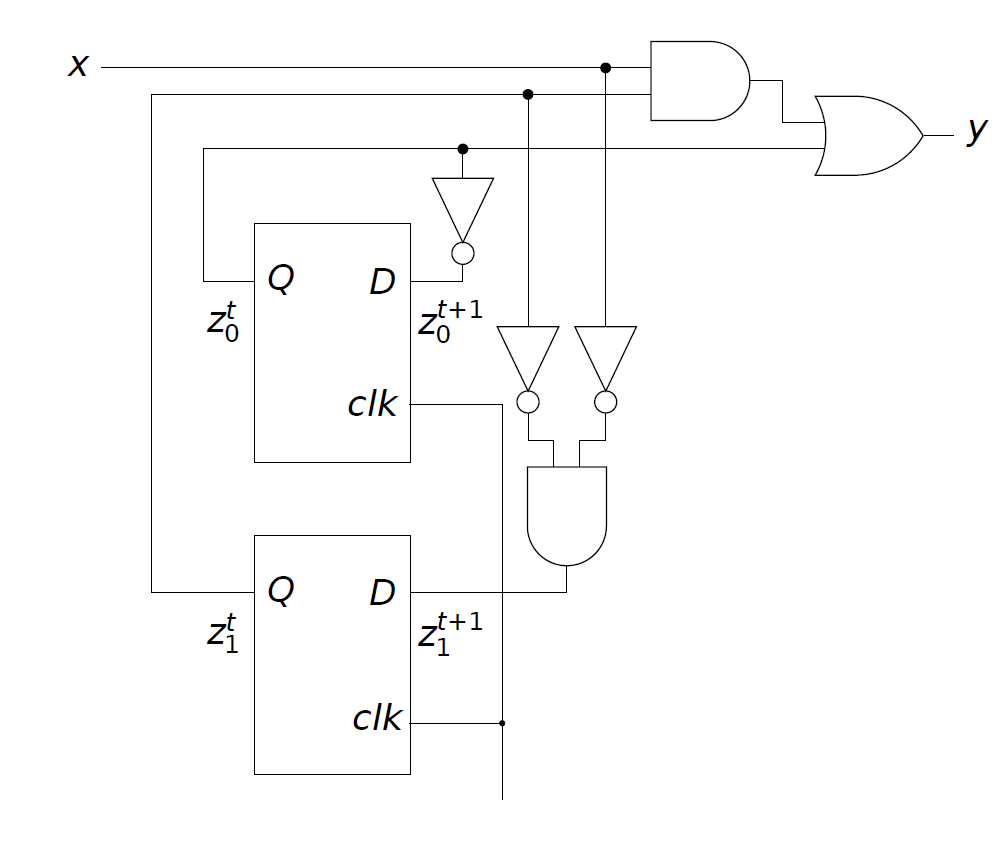
\includegraphics[scale = 0.2]{./figures/Mealy-reduziert-Schaltwerk.png}
                \end{itemize}
            \end{block}
        \end{column}
      \end{columns}
    \end{frame}

    \begin{frame}{Aufgabe 3}{}
        \begin{block}{Aufgabe}
            Zeichne Zustandsdiagramm von:\\
            Incrementer einer Binärzahl als Mealy-Atomat:
            \begin{itemize}
                \item niedrigstwertiges Bit wird zuerst gelesen
                \item auf das höchstwertige Bit folgt $\#\#$
                \item das erste $\#$ wird durch das Überlauf-Bit ersetzt, das zweite bleibt stehen
                \item Symbole nach der Endmarkierung sollen durch $\#$ ersetzt werden
            \end{itemize}
        \end{block}
    \end{frame}

    \begin{frame}{Aufgabe 3}
        \begin{block}{Lösung}
            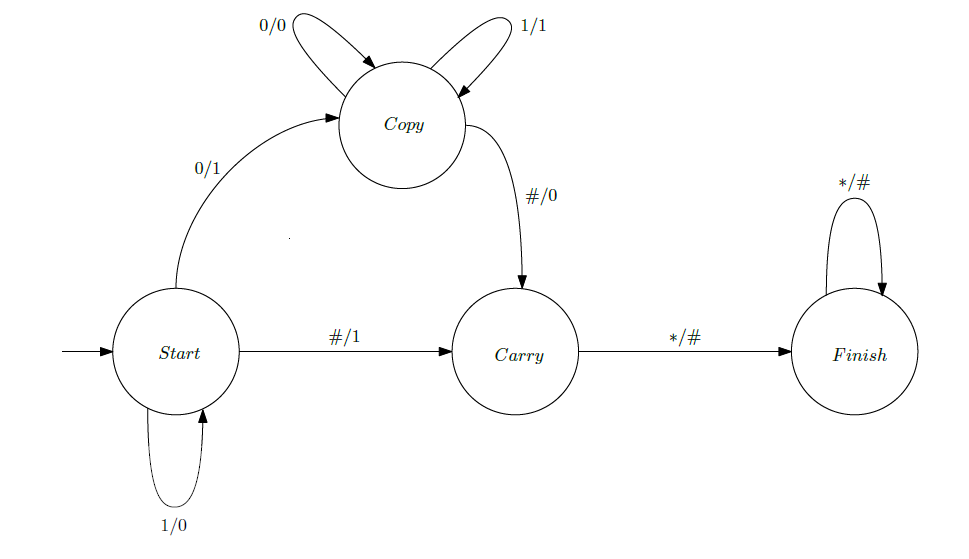
\includegraphics[scale=0.4]{./figures/Mealy-Increment.png}
        \end{block}
    \end{frame}

    \begin{frame}{Aufgabe 4}{}
      \begin{columns}
        \begin{column}{0.5\textwidth}
          \begin{block}{Aufgabe}
              \scriptsize
              Finde Gatter-Implementierung für \\$f$ und $g$ \\
              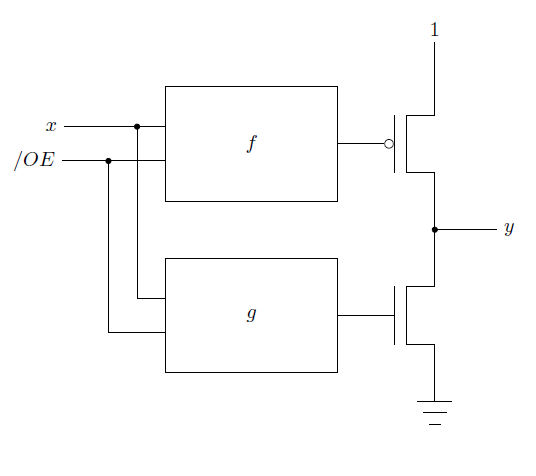
\includegraphics[scale=0.35]{./figures/Tristate-Treiber.png}
          \end{block}
        \end{column}
        \begin{column}{0.5\textwidth}
          \begin{block}{Lösung}
              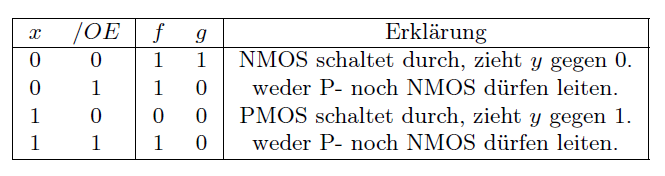
\includegraphics[scale=0.35]{./figures/Tristate-Treiber-Tabelle.png}\\
              \scriptsize
              $\Rightarrow f = \overline{x} \cdot \overline{/OE} + \overline{x} \cdot /OE + x \cdot /OE$ \\
              $ \ \ \ \ \ \  = \overline{x} + /OE$ \\
              $ \ \ \ \ \ \  = \overline{x \cdot \overline{ /OE}}$ \newline \newline \newline
              $\Rightarrow g = \overline{x} \cdot \overline{/OE} $ \\
              $ \ \ \ \ \ \  = \overline{x + /OE}$%\\$
          \end{block}
        \end{column}
      \end{columns}
    \end{frame}

    \begin{frame}{Aufgabe 4}{}
      \begin{columns}
        \begin{column}{0.5\textwidth}
          \begin{block}{Möglichkeit 1}
            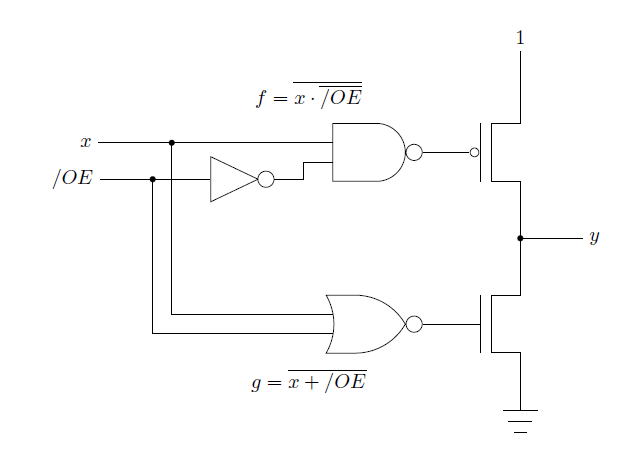
\includegraphics[scale=0.325]{./figures/Tristate-Treiber-Schlatkreis.png}
          \end{block}
        \end{column}
        \begin{column}{0.5\textwidth}
          \begin{block}{Möglichkeit  2}
            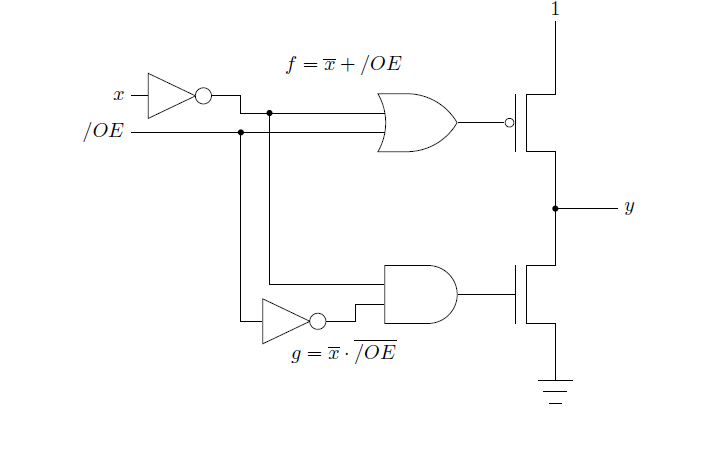
\includegraphics[scale=0.325]{./figures/Tristate-Treiber-Schlatkreis-Alternative.png}\\
          \end{block}
        \end{column}
      \end{columns}
    \end{frame}
 
\end{document}
